\part{Applied Partial Differential Equations}

\begin{multicols}{2}
An Ordinary Differential Equation (ODE) describes an \emph{unknown} function through its derivatives with respect to \emph{\textbf{single}} variable:
\begin{align*}
	m {d^2 x(t) \over d t^2} = F(x(t)).
\end{align*}
 A Partial Differential Equation (PDE) describes an unknown function through its partial derivatives with respect to \emph{\textbf{multiple}} variables:
 \begin{align*}
 	{\delta u(t, x) \over \delta t^2} = c^2 {\delta u(t, x) \over \delta4 x^2}.
 \end{align*}

\section{Example:} 1D Advection. Weather forecast: Simulate temperature evolution.
\begin{figure}[H]
	\centering
	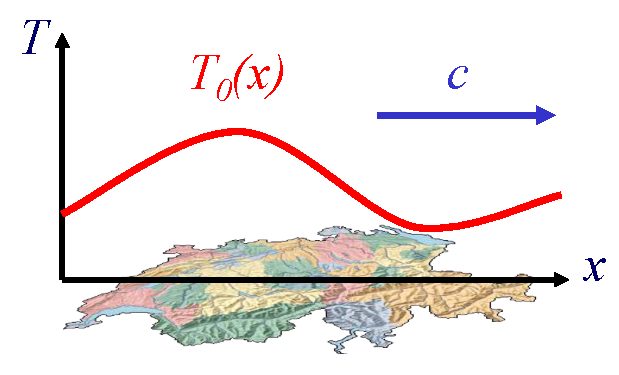
\includegraphics[width=0.45\textwidth]{img/03_weather}
\end{figure}
Given the temperature distribution $T_0(x)$ at time $t=0$ and wind speed $c$. Find an expression for the temperature evolution $T(x,t)$!

\subsection{Analytical Solution}

How does the temperature change over a time interval $\Delta  t$?
\begin{figure}[H]
	\centering
	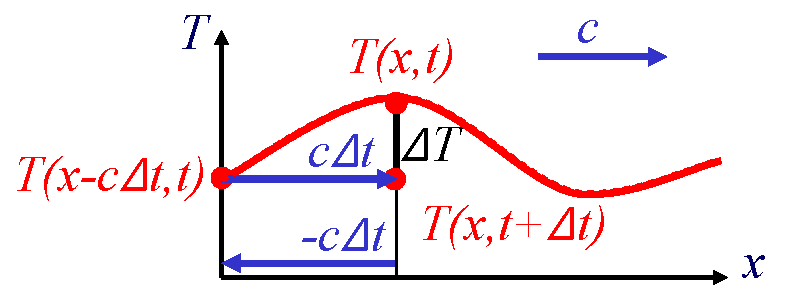
\includegraphics[width=0.45\textwidth]{img/03_1D_advection}
\end{figure}
\begin{align*}
	T(x, t+\Delta t) &= T(x-c\Delta t, t) \\
	\Delta T &= T(x,t+\Delta t) - T(x,t)\\
	T(x-c\Delta t, t) &= T(x,t) - {\partial T \over \partial x} c \Delta t + \bigO{\Delta t^2} = T(x, t+\Delta t)
\end{align*}

From which we can build the advection equation:
\begin{align*}
	{\Delta T  \over \Delta} t \approx -c {\partial T \over \partial x} \quad
	\lim_{\Delta \mapsto 0} \implies \quad {\partial T \over \partial t} = -c {\partial T \over \partial x}
\end{align*}
Any $T(x,t)$ of the form $T(x,t) = f(x-ct)$ solves ${\partial T \over \partial t} = -c {\partial T \over \partial x}$.  The solution also needs to satisfy the initial condition:
	\begin{align*}
		T(x,0) &= T_0(x)
	\end{align*}
	The solution is thus
	\begin{align*}
		T(x, t) &= T_0(x-ct)
	\end{align*}

\subsection{Numerical Solution}
Sample temperature $T(x,t)$ on 1D grid $T^t[i] = T(i\cdot h, t\cdot \Delta t)$ with $i \in (1,\ldots n)$, $t \in (0,1,2, \ldots)$:
\begin{figure}[H]
	\centering
	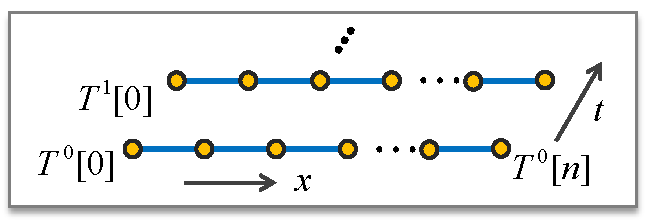
\includegraphics[width=0.45\textwidth]{img/03_numerical_solution}
	\caption{Sampling Grid}
\end{figure}

\section{Overview}
\begin{description}
	\item[Order of PDE] The \emph{order} of a PDE is the order of it's highest partial derivative.
	\item[Linearity] A PDE is \emph{linear} if the unknown function $(u)$ and it's partial derivatives only occure linearly:
		\begin{align*}
			\text{Linear example: }\ & u_t+c\cdot u_x = 0 & \text{(Advection eq.)}\\
			\text{Nonlinear example: }\ & u_t+u\cdot u = 0 & \text{(Burger's eq.)}
		\end{align*}
		Coefficients of linear PDEs can be nonlinear functions:
		\begin{align*}
			y^2 \cdot u_{yy} + x^2 \cdot u_{yy} = 0
		\end{align*}


\end{description}

\subsection{PDE Classification}
$2^{nd}$ order linear PDEs are of highest practical relevance. A $2^{nd}$ order linear PDE has the form:
\begin{align*}
	Au_{xx} + 2Bu_{xy} + Cu_{yy} = F(x,y,u, u_x, u_y).
\end{align*}
A $2^{nd}$ order linear PDE is either:
\begin{align*}
	\textbf{Hyperbolic}\quad B^2-AC > 0 &\text{Wave equation}\\
	\textbf{Parabolic}\quad B^2-AC = 0 &\text{Heat equation}\\
	\textbf{Elliptic}\quad B^2-AC < 0 &\text{Laplace equation}
\end{align*}

\begin{figure}[H]
	\centering
	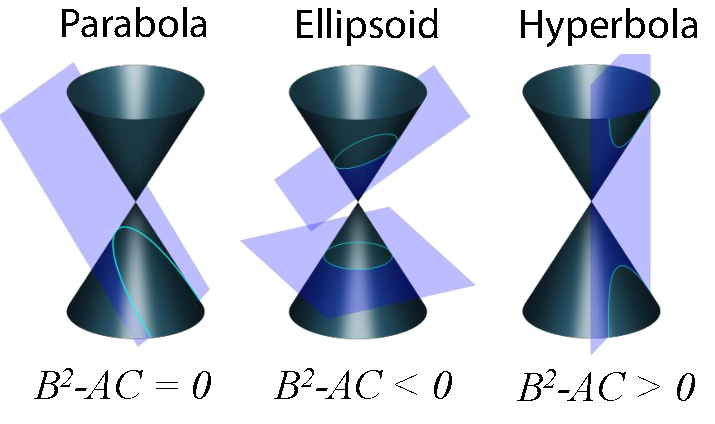
\includegraphics[width=0.45\textwidth]{img/03_PDE_classification}
\end{figure}

\subsection{Hyperbolic PDEs}
Hyperbolic PDEs are typically time dependent problems. They retain \& propagate disturbances present in initial data.
\paragraph{Prototype:} let $u$ be the amplitude and $c$ the propagation speed:
\begin{align*}
	\textbf{\emph{Wave Equation}:}\quad {\partial^2 u \over \partial t^2} = {\partial^2 u \over \partial x^2} c^2
\end{align*}
\paragraph{Applications}
\begin{itemize}
	\item Simulate wave propagation for sound, light and water.
	\item Mechanics: Oscillatory motion, vibrating strings.
\end{itemize}

\subsection{Parabolic PDEs}
Parabolic PDEs are typically time dependent problems. Solutions \emph{smooth out} as time increases.
\paragraph{Prototype:} let $u$ be the temperature and $\alpha$ the thermal diffusivity:
\begin{align*}
	\textbf{\emph{Heat Equation}:}\quad {\partial u \over \partial t} = \alpha {\partial^2 u \over \partial x^2}
\end{align*}

\paragraph{Application} consist of conduction and general diffusion processes.

\subsection{Elliptic PDEs}
Elliptic PDEs describe static problems (i.e. systems in equilibrium). Solutions are smooth (if the coefficients are).
\paragraph{Prototype:} 
\begin{align*}
	\textbf{\emph{Laplace Equation}:}\quad {\partial^2 u \over \partial x^2} + {\partial^2 u \over \partial y^2} = 0
\end{align*}

\paragraph{Applications} consist of steady-state solutions to hyperbolic and parabolic PDEs and of equilibrium problems.

\section{Boundary Conditions}
Generally there are (infinitely) many $u$ which solve a PDE. So there's additional information required $\rightarrow$ \emph{Boundary Conditions}. Typically $u$ is defined in a region $D$ and the solution is required to satisfy certain conditions on the boundary $\delta D$ of $D$:
\begin{figure}[H]
	\centering
	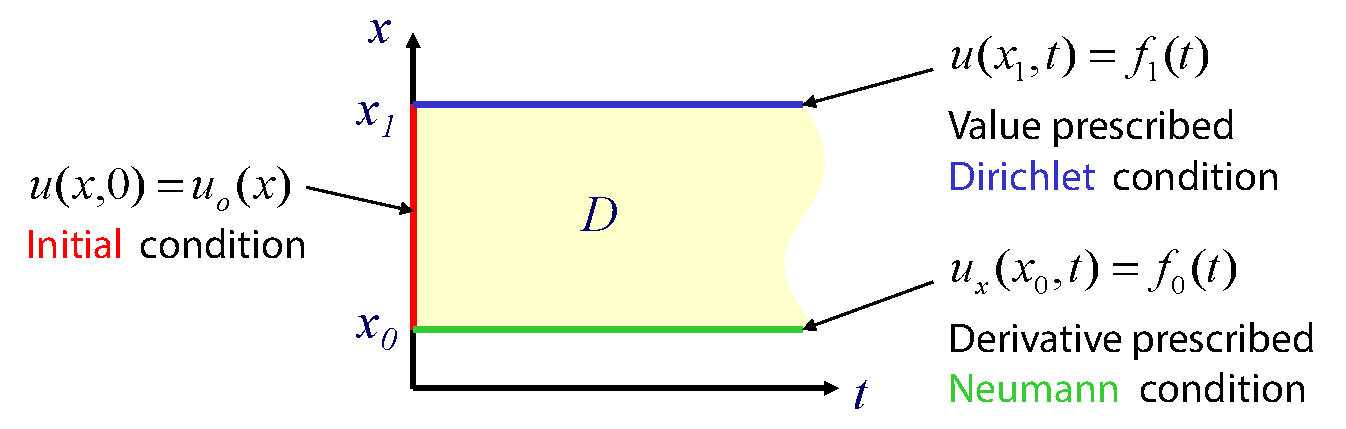
\includegraphics[width=0.45\textwidth]{img/03_boundary_conditions}
\end{figure}

\section{Solving Poisson's Equation Numerically}
\subsection{Poisson's Equation}
\begin{align*}
	-\Delta u(x,y) = f(x,y)
\end{align*}

The poisson equation is the same as Laplace Equation if $f(x,y) = 0$. The $2D$ Laplace operator:
\begin{align*}
	\Delta u(x,y) := {\partial^2 \over \partial x^2} u(x,y) + {\partial^2 \over \partial y^2} u(x,y)
\end{align*}

Poisson's equation has practical relevance:
\begin{itemize}
	\item \emph{Thin membrane} clamped at boundary (drum):
	
		$f(x,y)$ applies forces, $u(x,y)$ vertical displacement.
	\item \emph{Electrical potential} due to charge distribution:
		
		$f(x,y)$ charge distribution, $u(x,y)$ electric potential field.
		
	\item Steady state \emph{heat distribution}:
	
		$f(x,y)$ heat sources, $u(x,y)$ heat distribution.
\end{itemize}

\subsection{Finite Difference Solution}
Consider the 1D problem:
\begin{align*}
-u_{xx}(x) &= f(x) & x\in \Omega=(0,1)\\
u(0) &= 0\\
u(1) &= 0
\end{align*}

Use a regular grid to discretize $\Omega$:
\begin{align*}
	u[i] &= u(i\cdot h) &i \in (0, \ldots, n).
\end{align*}
Approximate derivatives with finite differences:
\begin{align*}
	u_{xx} = {u_x[i]-u_x[i-1] \over h} =  {u[i+1]-2u[i]+u[i-1] \over h}.
\end{align*}
Which gives us an equation for every grid point $i=2,\ldots, n-1$:
\begin{align*}
	h^2f[i] = u[i+1]-2u[i]+u[i+1]
\end{align*}


\paragraph{2D Finite Differences stencil}
\begin{align*}
	\Delta_h u[i,j] = {u[i+1,j] + u[i-1,j] + u[i, j-1] + u[i,j+1] - 4u[i,j] \over h^2}
\end{align*}


\paragraph{Problems and Drawbacks} Finite differences
\begin{itemize}
	\item Are easy to understand and implement
	\item require a regular grid
	\item high smoothness requirements on solution
	\item higher order derivatives require large stencils
\end{itemize}


\subsection{Finite Elements Solution}
Consider the 1D problem:
\begin{align*}
-u_{xx}(x) &= f(x) & x\in \Omega=(0,1)\\
u(0) &= 0\\
u(1) &= 0
\end{align*}

Assum the PDE is satisfied point wise then
\begin{align*}
	-\int_\Omega u_{xx} (x) dx = \int_\Omega f(x) dx,
\end{align*}
and also
\begin{align*}
	-\int_\Omega u_{xx} (x)\cdot v(x) dx = \int_\Omega f(x)\cdot v(x) dx
\end{align*}
where $v(x)$ is a testing function. For arbitrary smooth functions $v: \Omega \rightarrow \R$.

\paragraph{Weak Form} can be computed by using integration by parts:
\begin{align*}
	\int_a^b f'\cdot g = [f\cdot g]_a^b - \int_a^b f\cdot g'.
\end{align*}

\begin{align*}
	-\int_\Omega u_{xx} \cdot v dx &= \int_\Omega f \cdot v dx,\\
	\int_\Omega u_x \cdot v_x dx &= \int_\Omega f\cdot v + [u_x\cdot v]_0^1,\\
&\text{with } v(0) = v(1) = 0,
\end{align*}
we get the weak form:
\begin{align*}
	\int_\Omega u_x\cdot v_x dx = \int_\Omega f\cdot v dx.
\end{align*}
The \emph{order of the highest derivatives has decreased by one}. This function is called the \emph{weak form} since it imposes \emph{weaker} continuity requirements on the solution. The \emph{weak and strong forms are equivalent}.

\subsubsection{FEM-Template Process}
\begin{enumerate}
	\item Weak formulation
	\item Ritz-Galerkin approach
	\item Choice of Function Space 
	\item Geometric Decomposition of Domain
	\item Setup Matrix Equations
	\item Solve Linear System
\end{enumerate}

\subsubsection{Ritz-Galkerin Approach}
So far, $u(x)$ and $f(x)$ were continuous functions. We choose a finite-dimensional subspace for $u(x)$ and $f(x)$ and solve the projected problem (i.e. the weak form). 

We discretize $u$ and $v$ on $n$-dimensional space:
\begin{itemize}
	\item Sample with nodal positions $x_i$
	\item Nodal coefficients $u_i$
	\item Basis functions $N_i$
\end{itemize}
and get:
\begin{align*}
u(x) = \sum_i u_i N_i(x)
\end{align*}

\begin{figure}[H]
	\centering
	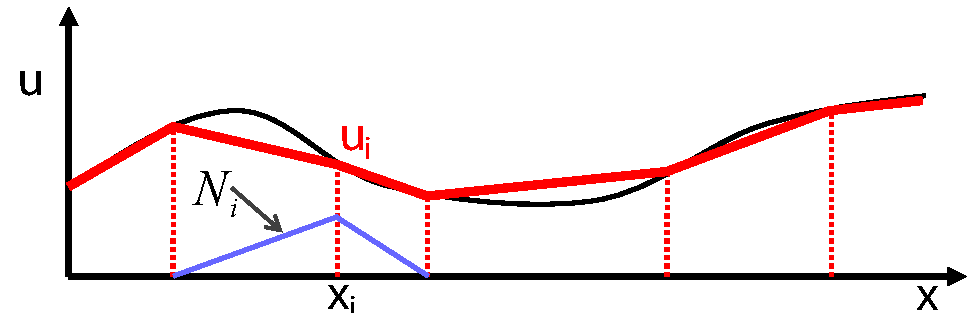
\includegraphics[width=0.45\textwidth]{img/03_galerkin_sampling}
\end{figure}


We observe that:
\begin{align*}
u(x) = \sum_i u_i N_i(x) \ \implies \ {\partial \over \partial x} u(x) = \sum_{i=1}^n  u_i  {\partial \over \partial x} N_i(x).
\end{align*}
Insert everything into the weak formulation:
\begin{align*}
	&\int_\Omega u_x v_x\ dx = \int_\Omega fv\ dx\\
	&\quad \int_\Omega \sum_{i=1}^n u_i {\partial N_i \over \partial x} \cdot \sum_{j=1}^n v_j {\partial N_j \over \partial x} dx - \int_\Omega f \cdot \sum_{j=1}^n v_j N_j(x)\ dx = 0
\end{align*}
Transform it:
\begin{align*}
	&\int_\Omega \sum_{i=1}^n u_i {\partial N_i \over \partial x} \cdot \sum_{j=1}^n v_j {\partial N_j \over \partial x} dx - \int_\Omega f \cdot \sum_{j=1}^n v_j N_j(x)\ dx = 0,\\
	&\sum_{j=1}^n v_j \left[\sum_{i=1}^n u_i \int_\Omega {\partial N_i \over \partial x} \cdot {\partial N_j \over \partial x} dx - \int_\Omega f \cdot N_j(x)\ dx \right] = 0.
\end{align*}
And we get $n$ linear equations for $n$ unknowns:
\begin{align*}
&\sum_{i=1}^n u_i \int_\Omega {\partial N_i \over \partial x} \cdot {\partial N_j \over \partial x} dx - \int_\Omega f \cdot N_j(x)\ dx = 0 &\forall i=1,\ldots, n
\end{align*}
Which can be written as a linear system $\mathbf{Ku} = \mathbf{f}$:
\begin{align*}
\underbrace{
\begin{pmatrix}
K_{11} & \cdots & K_{1n}\\
\vdots & \ddots & \vdots\\
K_{n1} & \cdots & K_{nn}
\end{pmatrix}}_\mathbf{K} \cdot  
\underbrace{
\begin{pmatrix}
u_1\\ \vdots \\ u_n
\end{pmatrix}
}_\mathbf{u}
= 
\underbrace{
\begin{pmatrix}
f_1\\ \vdots \\ f_n
\end{pmatrix}
}_\mathbf{f},
\end{align*}
where
\begin{align*}
	K_{ij} &= \int_\Omega {\partial N_i \over \partial x} {\partial N_j \over \partial x} dx,\\
	f_i &= \int_\Omega f\ N_i(x)dx.
\end{align*}

This matrix is
\begin{itemize}
	\item Symmetric
	\item Positive definite (elliptic PDE)
	\item Sparse (if $N_i$ has compact support)
\end{itemize}


\subsubsection{Choice of the Function Space}
Problem: What basis functions should be used in $u(x) = \sum_i u_i N_i(x)$?\\
Use piecewise linear basis functions. Basis functions are uniquely defined through \emph{Geometry} and interpolation requirement $N_i(x_j) = \delta_{ij}$.
\begin{figure}[H]
	\centering
	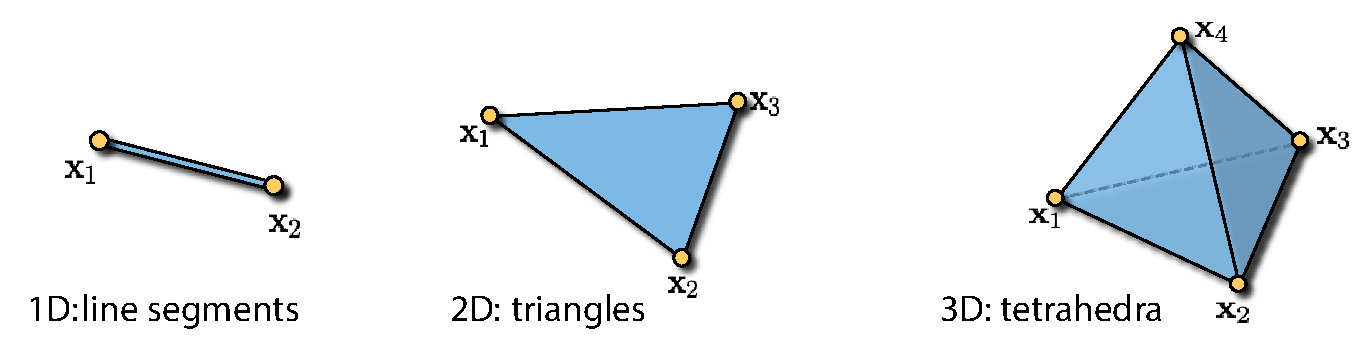
\includegraphics[width=0.45\textwidth]{img/03_elements}
	\caption{Simplical Elements}
\end{figure}

\paragraph{Triangle basis} $\text{}$
\begin{figure}[H]
	\centering
	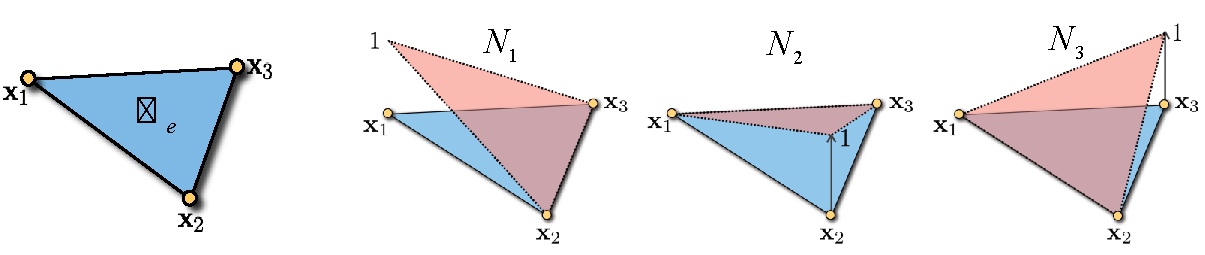
\includegraphics[width=0.45\textwidth]{img/03_triangle_basis}
\end{figure}
Basis functions: 
\begin{align*}
	N_i(x,y) = a_ix + b_iy + c.
\end{align*}
Due to $N_i(x_j) = \delta_{ij}$, we have:
\begin{align*}
	\begin{pmatrix}
		x_1 & y_1 & 1\\
		x_2 & y_2 & 1\\
		x_3 & y_3 & 1
	\end{pmatrix} \cdot
	\begin{pmatrix}
	a_i \\ b_i \\ c_i
	\end{pmatrix}
	= 
	\begin{pmatrix}
		\delta_{1i}\\
		\delta_{2i}\\
		\delta_{3i}
	\end{pmatrix}.
\end{align*}

\subsection{Finite Elements}
A finite element is a triple consisting of 
\begin{itemize}
	\item A closed subset $\Omega_e \subset \R^d$ (in $d$ dimensions)
	\item A set of $n$ basis functions: $N_i: \Omega_e \rightarrow \R$
	\item A set of $n$ associated nodal variables $x_i$.
\end{itemize}
In order to solve a PDE we need to know on how to tessellate a domain into elements:
\begin{itemize}
	\item 2D: Delaunay triangulator
	\item 3D: Tetrahedral mesher
\end{itemize}

\subsubsection{Integrating Basis Functions}
Goal: Evaluate $\mathbf f$
\begin{align*}
	f_i = \int_\Omega fN_idxdy
\end{align*}
$N_i$ extends over all $n_{e,i}$ elements incident to $x_i$. $N_i$ is zero outside of $\Omega_i \subset \Omega$. Evaluate integral over $\Omega_e$ with \emph{quadrature rule}:
\begin{align*}
	\int_{\Omega^e} f\ N_i^e\ dxdy &\approx f(x_q, y_q)\cdot N_i^e(x_q, y_q)\cdot A_e\\
	A_e:&\ \text{ Area of element } e\\
	(x_q, y_q):&\ \text{ single quadrature point at bary-center}
\end{align*}

Goal: Evaluate $\mathbf K$
\begin{align*}
	K_{ij} &= \int_\Omega {\partial N_i \over \partial x} {\partial N_j \over \partial x} + {\partial N_i \over \partial y} {\partial N_j \over \partial y} dx dy
\end{align*}
Observe that $K_{ij} \neq 0 \leftrightarrow \exists \Omega^e$ such that $\int_\Omega^e N_i^e N_j^e dxdy > 0$. Let $S_{ij}$ denote set of all these elements, then:
\begin{align*}
	K_{ij} &= \sum_{e \in S_{ij}} \int_\Omega {\partial N_i^e \over \partial x} {\partial N_j^e \over \partial x} 
	+ {\partial N_i^e \over \partial y} {\partial N_j^e \over \partial y} dx dy
\end{align*}
This allows for a element-centered implementation: For each element $e$:
\begin{itemize}
	\item Compute basis function derivatives: 
		\begin{align*}
			&{\partial N_l^e \over \partial x}&l=1,\ldots, 3
		\end{align*}
	\item Form products and integrate:
		\begin{align*}
			&{\partial N_l^e \over \partial x}{\partial N_k^e \over \partial x}&l=1,\ldots, 3\ k=1,\ldots, 3
		\end{align*}
	\item Add to global matrix:
		\begin{align*}
		K_{ij} +=  A_e \left( {\partial N_i^e \over \partial x} {\partial N_j^e \over \partial x} 
	+ {\partial N_i^e \over \partial y} {\partial N_j^e \over \partial y} \right)		\end{align*}
\end{itemize}

\subsubsection{Advantages of Finite Elements}
FEM $\{\ldots\}$
\begin{itemize}
	\item can easily deal with complex geometries,
	\item solution in nodes is naturally interpolated inside elements using basis functions
	\item weaker smoothness requirements on solution
	\item weak form is natural for many applications
	\item $\ldots$
\end{itemize}











\end{multicols}